% !TEX TS-program = pdflatex
% !TEX encoding = UTF-8 Unicode

% This file is a template using the "beamer" package to create slides for a talk or presentation
% - Giving a talk on some subject.
% - The talk is between 15min and 45min long.
% - Style is ornate.

% MODIFIED by Jonathan Kew, 2008-07-06
% The header comments and encoding in this file were modified for inclusion with TeXworks.
% The content is otherwise unchanged from the original distributed with the beamer package.

\documentclass{beamer}
\setbeamercovered{invisible}



% Copyright 2004 by Till Tantau <tantau@users.sourceforge.net>.
%
% In principle, this file can be redistributed and/or modified under
% the terms of the GNU Public License, version 2.
%
% However, this file is supposed to be a template to be modified
% for your own needs. For this reason, if you use this file as a
% template and not specifically distribute it as part of a another
% package/program, I grant the extra permission to freely copy and
% modify this file as you see fit and even to delete this copyright
% notice. 


\mode<presentation>
{
  \usetheme{Warsaw}
  % or ...

  % or whatever (possibly just delete it)
}


\usepackage[english]{babel}
% or whatever

\usepackage[utf8]{inputenc}
% or whatever

\usepackage{times}
\usepackage[T1]{fontenc}
% Or whatever. Note that the encoding and the font should match. If T1
% does not look nice, try deleting the line with the fontenc.

%%% MATH RELATED


%%% AMS math stuff
\usepackage{amsmath}
\usepackage{amssymb}
\usepackage{amsthm}
\usepackage{mathrsfs}
\usepackage{enumerate}

%%% Theorem environments
\newtheorem{thm}{Theorem}[subsection]
\newtheorem{prop}[thm]{Proposition}
\newtheorem{cor}{Corollary}[thm]
\newtheorem{por}[thm]{Porism}
\newtheorem{lem}[thm]{Lemma}
\theoremstyle{definition}
\newtheorem{prob}[thm]{Problem}
\newtheorem{soln}{Solution}
\newtheorem{defn}[thm]{Definition}
\newtheorem{ex}[thm]{Example}
\newtheorem{quest}[thm]{Question}
\newtheorem{remk}[thm]{Remark}

%%% Typesetting shortcuts
\newcommand{\tn}[1]{\textnormal{#1}}
\newcommand{\ol}[1]{\overline{#1}}
\newcommand{\wt}[1]{\widetilde{#1}}
\newcommand{\wh}[1]{\widehat{#1}}
\newcommand{\vocab}[1]{\textbf{#1}\index{#1}}

%%% Math shortcuts
\newcommand{\bbr}{\mathbb R}
\newcommand{\bbz}{\mathbb Z}
\newcommand{\bbq}{\mathbb Q}
\newcommand{\bbn}{\mathbb N}
\newcommand{\bbf}{\mathbb F}
\newcommand{\bbc}{\mathbb C}
\newcommand{\bbd}{\mathbb D}
\newcommand{\bba}{\mathbb A}
\newcommand{\bbp}{\mathbb P}
\newcommand{\bbg}{\mathbb G}
\newcommand{\bbv}{\mathbb V}
\newcommand{\dih}[1]{\mathcal D_{#1}}
\newcommand{\sym}[1]{\mathcal S_{#1}}
\newcommand{\vspan}{\tn{span}}
\newcommand{\trace}{\tn{trace}}
\newcommand{\diff}{\backslash}
\newcommand{\stab}{\tn{stab}}
\newcommand{\conv}{\tn{conv}}
\newcommand{\img}{\tn{img}}
\newcommand{\coker}{\tn{coker}}
\newcommand{\id}{\tn{id}}
\newcommand{\Hom}{\tn{Hom}}
\newcommand{\End}{\tn{End}}
\newcommand{\Aut}{\tn{Aut}}
\newcommand{\aut}{\tn{Aut}}
\newcommand{\ann}{\tn{Ann}}
\newcommand{\GL}{\tn{GL}}
\newcommand{\Gr}{\tn{Gr}}
\newcommand{\lord}{\preccurlyeq}
\newcommand{\rord}{\succcurlyeq}
\newcommand{\tr}{\textnormal{Tr}}
\newcommand{\Tr}{\textnormal{Tr}}
\newcommand{\bbl}{\mathbb{L}}
\newcommand{\C}{\mathscr{C}}
\newcommand{\X}{\mathscr{X}}
\renewcommand{\S}{\mathscr{S}}
\newcommand{\M}{\mathscr{M}}
\renewcommand{\L}{\mathcal{L}}


%%% Algebraic Geometry
\newcommand{\height}{\textnormal{ht}}
\newcommand{\A}{\mathbb{A}}
\newcommand{\p}{\mathfrak{p}}
\newcommand{\sheaf}[1]{\mathcal{#1}}
\newcommand{\spec}{\textnormal{Spec}}
\newcommand{\proj}{\textnormal{Proj}}
\newcommand{\Aff}{\textnormal{Aff}}
\newcommand{\skel}{\textnormal{skel}}
\newcommand{\supp}{\textnormal{supp}}
\newcommand{\orb}{\textnormal{orb}}
\newcommand{\Proj}{\textnormal{Proj}}
\newcommand{\Pic}{\textnormal{Pic}}
\newcommand{\Rees}{\textnormal{Rees}}
\newcommand{\shom}{\mathcal{H}om}

\renewcommand*\arraystretch{1.3}

%%% paper specific definitions
\newcommand{\weyl}{\Omega}
\newcommand{\weyll}{{\widehat{\Omega}}}
\newcommand{\weylll}{{\widetilde{\Omega}}}
\newcommand{\mweyl}{{M_N(\Omega)}}
\newcommand{\mweyll}{{M_N(\widehat{\Omega})}}
\newcommand{\mweylll}{{M_N(\widetilde{\Omega})}}
\newcommand{\seq}{\text{Seq}}
\newcommand{\tail}{\text{Tail}}
\newcommand{\Ad}{\textnormal{Ad}}
\newcommand{\sech}{\textnormal{sech}}
\newcommand{\colim}{\varinjlim}
\newcommand{\limit}{\varprojlim}
\newcommand{\Bis}{\textnormal{Bis}}
\newcommand{\m}{\mathfrak{m}}
\newcommand{\mxx}[4]{\left(\begin{array}{cc} #1 & #2\\ #3 & #4 \end{array}\right)}
\newcommand{\diag}{\text{diag}}
\newcommand{\qdet}{\textnormal{qdet}}
\newcommand{\mdet}{\textnormal{mdet}}
\newcommand{\mtau}{\mathcal{T}}
\newcommand{\cof}{\textnormal{cof}}
\newcommand{\minor}{\textnormal{minor}}
\newcommand{\holo}{Holo}
\newcommand{\ord}{\textnormal{order}}
\newcommand{\mult}{\mathfrak M}






\title{MATH 350-2 Advanced Calculus} 
\subtitle
{} % (optional)

\author[W.R. Casper] % (optional, use only with lots of authors)
{W.R. Casper}
% - Use the \inst{?} command only if the authors have different
%   affiliation.

\institute[California State University Fullerton] % (optional, but mostly needed)
{
  Department of Mathematics\\
  California State University Fullerton}
% - Use the \inst command only if there are several affiliations.
% - Keep it simple, no one is interested in your street address.

\subject{Talks}
% This is only inserted into the PDF information catalog. Can be left
% out. 



% If you have a file called "university-logo-filename.xxx", where xxx
% is a graphic format that can be processed by latex or pdflatex,
% resp., then you can add a logo as follows:

% \pgfdeclareimage[height=0.5cm]{university-logo}{university-logo-filename}
% \logo{\pgfuseimage{university-logo}}



% Delete this, if you do not want the table of contents to pop up at
% the beginning of each subsection:
\AtBeginSubsection[]
{
  \begin{frame}<beamer>{Outline}
    \tableofcontents[currentsection,currentsubsection]
  \end{frame}
}


% If you wish to uncover everything in a step-wise fashion, uncomment
% the following command: 

%\beamerdefaultoverlayspecification{<+->}


\begin{document}

\begin{frame}
  \titlepage
\end{frame}

\begin{frame}{Outline}
  \tableofcontents
  % You might wish to add the option [pausesections]
\end{frame}

% Since this a solution template for a generic talk, very little can
% be said about how it should be structured. However, the talk length
% of between 15min and 45min and the theme suggest that you stick to
% the following rules:  

% - Exactly two or three sections (other than the summary).
% - At *most* three subsections per section.
% - Talk about 30s to 2min per frame. So there should be between about
%   15 and 30 frames, all told.

\section{Real Analysis Lecture 12}
\subsection{Metric Spaces}

\begin{frame}{Warm-up Challenge}
\begin{prob}
Write down each of the following:
\begin{itemize}
\item the definition of an open cover of a set $A$
\pause
\item a compact set
\pause
\item Lindel\"of Covering Theorem
\pause
\item Bolzano-Weierstrass Theorem
\pause
\item Cantor Intersection Theorem
\pause
\item Heine-Borel Theorem
\end{itemize}
\end{prob}
\end{frame}

\begin{frame}{Metric space}
\pause
\begin{defn}
A \vocab{metric space} is a pair $(M,d)$ consisting of a nonempty set $M$ of ``points", along with a distance function $d: M\times M\rightarrow\mathbb{R}$ with the following four properties.
\pause
\begin{enumerate}[\text{A}1]
\pause
\item $d(x,x) = 0$ for all $x\in M$
\pause
\item \textbf{positivity:}  $d(x,y) > 0$ for all $x,y\in M$ with $x\neq y$
\pause
\item \textbf{symmetry:}  $d(x,y) = d(y,x)$ for all $x,y\in M$
\pause
\item \textbf{triangle inequality:} $d(x,y)\leq d(x,z) + d(z,y)$ for all $x,y,z\in M$
\end{enumerate}
\end{defn}
\pause
The value $d(x,y)$ is called a \textbf{metric} and describes the ``distance" between $x$ and $y$.
\end{frame}

\begin{frame}{Open balls}
\pause
\begin{defn}
Let $(M,d)$ be a metric space.
The open ball of radius $r>0$ centered at $x\in M$ is
$$B_M(x;r) = \{y\in M: d(x,y) < r\}.$$
\end{defn}
\end{frame}

\begin{frame}{Examples of metrics on $\mathbb{R}^2$}
$$d_{\text{eucl}}(\vec x,\vec y) = |\vec x - \vec y| = \sqrt{(x_1-y_1)^2 + (x_2-y_2)^2}$$
\begin{itemize}
\pause
\item Euclidean metric (2-norm)
\pause
\item open balls are circles
\end{itemize}
\pause
\begin{center}
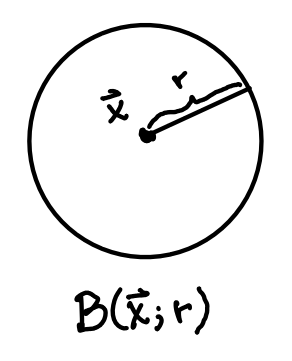
\includegraphics[height=1in]{fig/ball2.png}
\end{center}
\end{frame}

\begin{frame}{Examples of metrics on $\mathbb{R}^2$}
$$d_{\text{taxi}}(\vec x,\vec y) = |x_1-y_1| + |x_2-y_2|$$
\begin{itemize}
\pause
\item Taxi-cab metric ($1$-norm, distances on city streets)
\pause
\item open balls are diamonds
\end{itemize}
\pause
\begin{center}
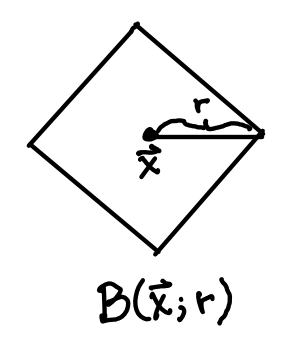
\includegraphics[height=1in]{fig/ball1.png}
\end{center}
\end{frame}

\begin{frame}{Examples of metrics on $\mathbb{R}^2$}
$$d_{\infty}(\vec x,\vec y) = \max\{|x_1-y_1|,|x_2-y_2|\}$$
\begin{itemize}
\pause
\item Chebyshev metric (infinity norm)
\pause
\item open balls are squares
\end{itemize}
\pause
\begin{center}
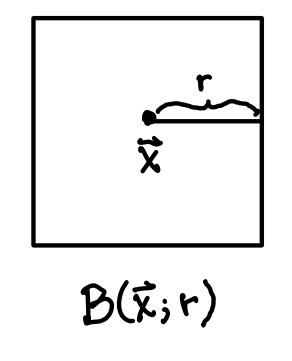
\includegraphics[height=1in]{fig/ballinf.png}
\end{center}
\end{frame}

\begin{frame}{Examples of metrics on $\mathbb{R}^2$}
$$d_p(\vec x,\vec y) = \sqrt[p]{|x_1-y_1|^p + |x_2-y_2|^p}$$
\begin{itemize}
\pause
\item $p$-norm, $1\leq p < \infty$
\pause
\item open balls are rounded squares
\end{itemize}
\pause
\begin{center}
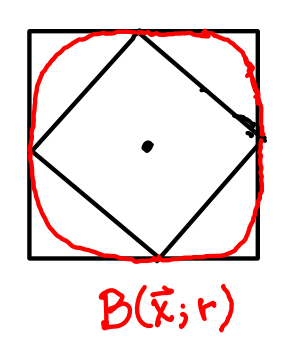
\includegraphics[height=1in]{fig/ballp.png}
\end{center}
\end{frame}

\begin{frame}{Challenge!}
Let $M$ be a nonempty set and define $d: M\times M\rightarrow \mathbb{R}$ by
$$d_{\text{disc}}(x,y) = \left\lbrace\begin{array}{cc}
1 &  x\neq y\\
0 &  x = y
\end{array}\right.$$
\pause
\begin{prob}
Prove that $d_{\text{disc}}$ is a metric.
\end{prob}
\pause
This is called the \textbf{discrete metric}.
\end{frame}

\begin{frame}{Challenge!}
\begin{prob}
What do the open balls with the discrete metric look like?
\end{prob}
\end{frame}

\begin{frame}{Open sets}
\begin{defn}
\pause
Let $(M,d)$ be a metric space and $A\subseteq M$.\\
\pause
A point $x\in M$ is called an \textbf{interior point} if there exists $r>0$ such that $B_M(x;r)\subseteq M$.\\
\pause
The set $\text{int}(A)$ of interior points of $A$ is called the \textbf{interior} of $A$.\\
\pause
The set $A$ is \textbf{open} if every point in $A$ is an interior point, or equivalently $\text{int}(A) = A$.
\end{defn}
\end{frame}

\begin{frame}{Challenge!}
\begin{prob}
Consider the metric space $(\mathbb{R},d_{\text{disc}})$ where $d_{\text{disc}}$ is the discrete metric.\\
What sets are open sets?
\end{prob}
\end{frame}

\begin{frame}{Closed sets}
\begin{defn}
\pause
Let $(M,d)$ be a metric space and $A\subseteq M$.\\
\pause
A set $A\subseteq M$ is closed if the complement $M\backslash A$ is open.\\
\pause
A point $ x\in M$ is an \vocab{adherent point} if for all $r>0$ the ball $B_M( x; r)$ contains an element of $M$.\\
\pause
A point $ x\in M$ is an \vocab{accumulation point} if for all $r>0$ the ball $B_M( x; r)$ contains an element of $M$ different from $x$.\\
\pause
The set $\overline M$ of all adherent points of $M$ is called the \vocab{closure} of $M$.
\end{defn}
\end{frame}


\begin{frame}{Challenge!}
\begin{prob}
Consider the metric space $(\mathbb{R},d_{\text{disc}})$ where $d_{\text{disc}}$ is the discrete metric.\\
Which sets are closed?
\end{prob}
\end{frame}

\begin{frame}{Challenge!}
\begin{prob}
Prove the following (Apostol Theorem 3.36).
If $(M,d)$ is a metric space, $U\subseteq M$ is open, and $C\subseteq M$ is closed, then $U\backslash C$ is open and $C\backslash U$ is closed.
\end{prob}
\end{frame}

\begin{frame}{Characterizing closed sets}
\begin{thm}[Apostol Theorem 3.37]
Let $(M,d)$ be a metric space and $A\subseteq S$.  Then the following are equivalent:
\begin{enumerate}[(a)]
\pause
\item $A$ is closed
\pause
\item $A$ contains all of its adherent points
\pause
\item $A$ contains all of its accumulation points
\pause
\item $A=\overline{A}$
\end{enumerate}
\end{thm}
\end{frame}


\begin{frame}{Unions and intersections}
\pause
\begin{thm}
Let $(M,d)$ be a metric space and  $\{U_i: i\in I\}$ be a family of open sets in $M$.
The union $\bigcup_{i\in I} U_i$ is open.
\end{thm}
\pause
\begin{proof}
Identical to the proof for $\mathbb{R}^n$.
\end{proof}
\pause
\begin{thm}
Let $(M,d)$ be a metric space and $U_1,U_2,\dots, U_n$ be open sets in $M$.
The intersection $\bigcap_{i=1}^n U_i$ is open.
\end{thm}
\pause
\begin{proof}
Identical to the proof for $\mathbb{R}^n$.
\end{proof}
\end{frame}

\begin{frame}{Unions and intersections}
\pause
\begin{thm}
Let $(M,d)$ be a metric space and  $\{C_i: i\in I\}$ be a family of closed sets in $M$.
The intersection $\bigcap_{i\in I} C_i$ is closed.
\end{thm}
\pause
\begin{proof}
Apply De Morgan's Laws.
\end{proof}
\pause
\begin{thm}
Let $(M,d)$ be a metric space and $C_1,C_2,\dots, C_n$ be closed sets in $M$.
The intersection $\bigcup_{i=1}^n C_i$ is closed.
\end{thm}
\pause
\begin{proof}
Apply De Morgan's Laws.
\end{proof}
\end{frame}

\subsection{Subspaces}

\begin{frame}{Metric subspace}
\begin{defn}
Let $(M,d)$ be a metric space.\\
\pause
If $S\subseteq M$ is a subset, then $d: M\times M\rightarrow \mathbb{R}$ restricts to a metric $d: S\times S\rightarrow \mathbb{R}$, called the \vocab{relative metric}.\\
\pause
The space $(S,d)$ with the relative metric is called a \vocab{metric subspace}.
\end{defn}
\pause
Open balls in $S$:
$$B_S(x; r) = B_M(x; r) \cap S.$$
\end{frame}

\begin{frame}{Open sets in subspaces}
\begin{thm}
Let $(M,d)$ be a metric space and let $(S,d)$ be a subspace.
Then $V$ is an open subset of $S$ if and only if there exists an open subset $U$ of $M$ with $V = U\cap S$.
\end{thm}
\pause
\begin{proof}
\pause
$\Longrightarrow$: Assume $V$ is an open subset of $S$.\\
\pause
Then for all $x\in V$, there exists $r_x>0$ such that $B_S(x;r_x) \subseteq V$.\\
\pause
This says $B_M(x; r_x)\cap S\subseteq V$.\\
\pause
Define
$$U = \bigcup_{x\in V} B_M(x;r_x).$$
\pause
This is a union of open sets, and is therefore open.
\pause
Furthermore $U\cap S = V$.
\end{proof}
\end{frame}

\begin{frame}{Open sets in subspaces}
\begin{thm}
Let $(M,d)$ be a metric space and let $(S,d)$ be a subspace.
Then $V$ is an open subset of $S$ if and only if there exists an open subset $U$ of $M$ with $V = U\cap S$.
\end{thm}
\pause
\begin{proof}
\pause
$\Longleftarrow$: Assume $U$ is an open subset of $M$.\\
\pause
We need to show that $V:= U\cap S$ is open.\\
\pause
If $x\in V$, then $x\in U$ and there exists $r>0$ such that $B_M(x;r)\subseteq U$.\\
\pause
It follows that $B_S(x,r) = B_M(x,r)\cap S\subseteq U\cap S = V$.\\
\pause
This shows that $x$ is an interior point of $S$ in the metric subspace $(S,d)$.\\
\pause
Since $x\in V$ was arbitrary, this shows that $V$ is open in $S$.
\end{proof}
\end{frame}

\begin{frame}{Closed sets in subspaces}
\begin{thm}
Let $(M,d)$ be a metric space and let $(S,d)$ be a subspace.
Then $B$ is a closed subset of $S$ if and only if there exists a closed subset $A$ of $M$ with $B = A\cap S$.
\end{thm}
\pause
\begin{proof}
\pause
Let $B\subseteq S$.\\
\pause
$B$ is closed in $S$ if and only if $S\backslash B$ is open in $B$\\
\pause
This is true if and only if there exists an open subset $U$ of $M$ with $S\backslash B = U\cap S$.\\
\pause
This is true if and only if there exists an open subset $U$ of $M$ with $B = (M\backslash U)\cap S$.\\
\pause
this is true if and only if there exists a closed subset $A$ of $M$ with $B = A\cap S$.
\end{proof}
\end{frame}

\begin{frame}{Example}
Consider the metric space $(\mathbb{R},d)$ with $d = d_{\text{eucl}}$ the Euclidean metric, and the metric subspace $(S,d)$ for $S = [0,1]$.
\begin{itemize}
\pause
\item $[0,1]$ is open in $S$ and closed in $S$, but it is not open in $M$
\pause
\item $[0,1/2)$ is open in $S$, but not in $M$
\pause
\item $(0,1/2)$ is open in both $S$ and in $M$
\pause
\item $(1/2,1]$ is open in $S$, but not in $M$
\end{itemize}
\end{frame}




\end{document}


